
%(BEGIN_QUESTION)
% Copyright 2012, Tony R. Kuphaldt, released under the Creative Commons Attribution License (v 1.0)
% This means you may do almost anything with this work of mine, so long as you give me proper credit

In this process, nitric acid and ammonia vapor are combined to form a chemical called {\it ammonium nitrate}, a key ingredient in synthetic fertilizer.  The ``scrubber'' vessel (V-5) uses a liquid spray to remove volatile chemical compounds from vapors before they exit out of an exhaust stack and into the atmosphere.  As water evaporates from this liquid solution due to the heat of the vapors, a ``make-up'' system (loop \#35) must add water to maintain a constant liquid level at the bottom of the scrubber vessel:

$$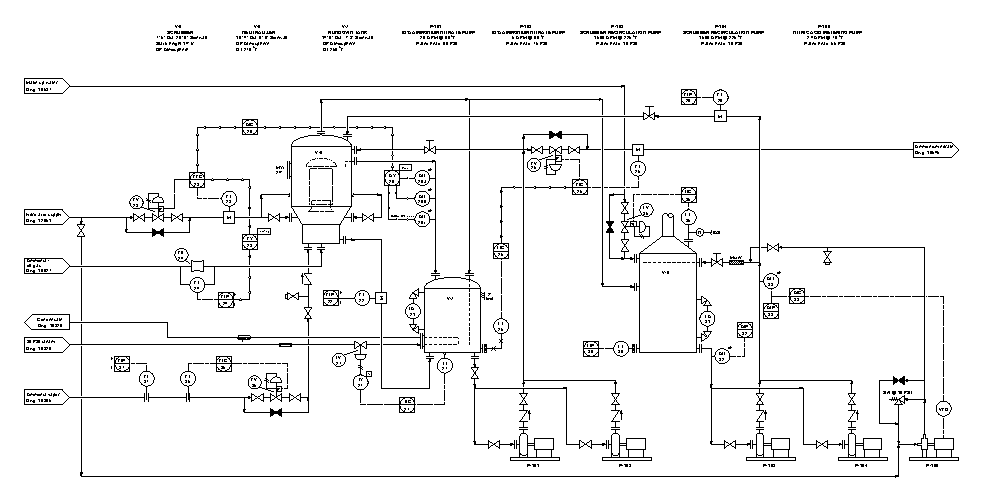
\includegraphics[width=15.5cm]{i0008rx01.eps}$$

Suppose the last instrument technician to calibrate the positioner on the level control valve (LV-35) made a mistake, and the valve position is consistently open 10\% more than it should be.  For example, if controller LIC-35 sends a 50\% (12 mA) control signal to the valve, the valve stem will settle at a position of 60\% open instead.

\vskip 10pt

Describe in detail the effect this mis-calibration will have on the performance of the level control system for the scrubber vessel.

\vskip 20pt \vbox{\hrule \hbox{\strut \vrule{} {\bf Suggestions for Socratic discussion} \vrule} \hrule}

\begin{itemize}
\item{} Perform a ``thought experiment'' where you put on a pair of shoes with much thicker soles than you are accustomed to before driving a car.  The extra thickness of your shoes' soles results in the accelerator pedal being pressed down further than it would normally be for any given foot position.  How will this affect your actual driving speed as you attempt to obey the speed limit?
\item{} Is the scrubber vessel in danger of over- or under-filling from the valve's mis-calibration?
\item{} Which would be more dangerous or destructive in this process: an over-filled scrubber or an under-filled scrubber? 
\item{} What purpose does a ``positioner'' serve on a control valve?
\end{itemize}

\underbar{file i02929}
%(END_QUESTION)





%(BEGIN_ANSWER)


%(END_ANSWER)





%(BEGIN_NOTES)

There will be no effect on the performance of this level control system, except in circumstances where the controller tries to completely shut the valve.  In those cases, the valve will still remain slightly open, and the liquid level in the scrubber will rise higher than it should.  During normal operation, however, the controller will still be able to maintain the scrubber's liquid level at setpoint.













\filbreak \vskip 20pt \vbox{\hrule \hbox{\strut \vrule{} {\bf Virtual Troubleshooting} \vrule} \hrule}

\noindent
{\bf Predicting the effect of a given fault:} present each of the following faults to the students, one at a time, having them comment on all the effects each fault would produce.

\begin{itemize}
\item{} 30 PSI steam supply fails
\item{} FT-36 fails with high signal
\item{} LT-35 fails with low signal
\item{} LT-26 fails with low signal
\item{} AIT-33 fails with high signal
\item{} Power fails to VFD on nitric acid pump
\end{itemize}


\vskip 10pt


\noindent
{\bf Identifying possible/impossible faults:} present symptoms to the students and then have them determine whether or not a series of suggested faults could account for all the symptoms, explaining {\it why} or {\it why not} for each proposed fault:

\begin{itemize}
\item{} Symptom: {\it }
\item{}  -- {\bf Yes/No}
\item{}  -- {\bf Yes/No}
\item{}  -- {\bf Yes/No}
\end{itemize}


\vskip 10pt


\noindent
{\bf Determining the utility of given diagnostic tests:} present symptoms to the students and then propose the following diagnostic tests one by one.  Students rate the value of each test, determining whether or not it would give useful information (i.e. tell us something we don't already know).  Students determine what different results for each test would indicate about the fault, if anything:

\begin{itemize}
\item{} Symptom: {\it }
\item{}  -- {\bf Yes/No}
\item{}  -- {\bf Yes/No}
\end{itemize}


\vskip 10pt


\noindent
{\bf Diagnosing a fault based on given symptoms:} imagine the ??? fails ??? in this system (don't reveal the fault to students!).  Present the operator's observation(s) to the students, have them consider possible faults and diagnostic strategies, and then tell them the results of tests they propose based on the following symptoms, until they have properly identified the nature and location of the fault:

\begin{itemize}
\item{} {\it }
\item{} 
\item{} 
\end{itemize}
%INDEX% Basics, control loop troubleshooting: determining effect of specified fault(s)
%INDEX% Process: ammonium nitrate production (realistic P&ID shown)

%(END_NOTES)


